% !TeX root = ../all.tex


\section{A General Algorithm}\label{sect:alg}

We present an algorithm for pure exploration in bandits with upper bounds on both its batch and sample complexities.
We take inspiration from the Track-and-Stop method \citep{garivierOptimalBestArm2016}, which is fully sequential (it does not use batches) and has asymptotically optimal sample complexity.
The principle of Track-and-Stop for Gaussians is to try to sample according to $w^\star(\bm\mu)=\argmax_{\bm w\in \Delta_K} \inf_{\bm{\lambda} \in Alt_{\bm{\mu}}} \sum_i w_i (\mu_i -\lambda_i)^2/(2\sigma^2)$, the vector of ideal sampling proportions at $\bm\mu$. At time $t$, having sampled arm $i$ approximately $w^\star_i t$ times leads to an algorithm that has minimal asymptotic sample complexity.
Of course $w^\star(\bm\mu)$ is unknown: Track-and-Stop estimates $\bm\mu$ by its empirical mean $\bm{\hat{\mu}}$, then approximates $w^\star(\bm\mu)$ by $w^\star(\bm{\hat{\mu}})$ and uses those proportions.
Some amount of uniform exploration is added to ensure convergence of the estimates.



We introduce a batched algorithm that first samples uniformly until it has estimated the sampling proportions and complexity well enough, then uses a last phase in which it samples like Track-and-Stop.

\subsection{Stopping Rule}

To check whether we can stop, a commonly used method in parametric pure exploration is the Generalized Likelihood Ratio (GLR) test \citep{garivierOptimalBestArm2016}.
Since we consider the non-parametric class of sub-Gaussian distributions, we use a Gaussian version of that test.
The stopping rule of the algorithm is to stop at the end of a phase if
\begin{equation}\label{eq:stop}
	\inf_{\bm\lambda \in Alt_{\hat{\bm\mu}^t} } \sum_i N_i^t\frac{(\hat{\mu}_i^t-\lambda_i)^2}{2\sigma^2} >\beta(t,\delta)
	\: .
\end{equation}

\begin{lemma}[\citep{garivierOptimalBestArm2016}]\label{lem:beta}
	Any algorithm using the stopping rule \eqref{eq:stop} with a threshold $\beta(t, \delta)$ satisfying
	$\mathbb{P}\left(\exists t,\sum_{i=1}^K N_i^t \frac{(\hat{\mu}_i^t-\mu_i)^2}{2\sigma^2} >\beta(t,\delta)\right) \le \delta$ and returning $i^\star(\hat{\bm\mu}^t)$ is $\delta$-correct.	
\end{lemma} 

We provide below a threshold that works for sub-Gaussian distributions in any pure exploration problem. For particular problems like BAI it should be possible to derive improved thresholds, as was done in parametric cases by \citet{kaufmannMixtureMartingalesRevisited2021}.
Our threshold is derived using the method of mixtures, as in that paper and other bandit articles \citep{abbasi2011improved}. It uses the techniques of \citep{degenneImpactStructureDesign2019} to fine-tune the constants.
While the BAI literature contains many similar thresholds for parametric settings, we could not find that result for sub-Gaussian distributions.

Let $W_{-1}$ be the negative branch of the Lambert $W$ function and let $\overline{W}:(1,+\infty) \to \mathbb{R}$ be the function defined by $\overline{W}(x) = -W_{-1}(-e^{-x})$. 
It satisfies $x + \ln x \le \overline{W}(x) \le x + \ln x + 1/2 \le 2x$.

\begin{lemma}\label{lem:beta_subG}
The following threshold satisfies the condition of Lemma~\ref{lem:beta} for $\sigma^2$-sub-Gaussian distributions:
\begin{align*}
\beta(t, \delta)
&= \frac{K}{2} \overline{W}\left(\frac{2}{K}\ln \frac{1}{\delta} + 4\ln \left(\ln \frac{et}{K}\right) + 2\ln \frac{e\pi^2}{6} \right)
\: .
\end{align*}
\end{lemma}

See Appendix~\ref{app:concentration} for the proof.
Roughly, ignoring additive constants, $\beta(t, \delta) \approx \ln(1/\delta) + 2K \ln\ln t$~.
The linear dependence in $K$ may be unavoidable in general (for the problem of telling if the means belong to the unit ball, if $\bm\mu$ is the center) but could be improved in problems like BAI. The threshold for exponential families of \citep{kaufmannMixtureMartingalesRevisited2021} depends logarithmically on the number of arms.



\subsection{Known Confidence Set}

In order to design an algorithm, we first ask the following questions: given enough information, could we return a correct answer within one batch? How would we sample and what would be the sample complexity?

Suppose that we know a set $B$ which likely contains $\bm\mu$ and will likely contain the empirical mean vector $\hat{\bm\mu}_t$ for any amount of sampling we perform.
Since we will be using only one batch, we have to select the number of samples for each arm in advance.
We want that number of samples to be sufficient to enable the stopping rule, for any $\bm\mu' \in B$.
Our solution will be based on two worst-case definitions.


\begin{definition}
	For any $B$ a set of instances, define (with $0^{-1} = +\infty$)
	\begin{align*}
	\overline{w}^\star(B) &= \argmax_{w\in \Delta_K} \inf_{\bm\nu \in B} \inf_{\bm\lambda\in Alt_{\bm\nu}} \sum_i w_i \frac{(\nu_i - \lambda_i)^2}{2 \sigma^2}
	\: , \\
	\overline{T}^\star(B) &= \left(\max_{w\in \Delta_K} \inf_{\bm\nu \in B} \inf_{\bm\lambda\in Alt_{\bm\nu}} \sum_i w_i \frac{(\nu_i - \lambda_i)^2}{2 \sigma^2}\right)^{-1}
	\: .
	\end{align*}
\end{definition}

Note that $\overline{T}^\star(B) \ge \max_{\bm\mu\in B} T^\star(\bm\mu)$ , but those two quantities may not be equal. To see this, imagine an instance $\bm\nu$ such that $w_i(\bm\mu)\neq w_j(\bm\mu)$, and instance $\bm\nu'$ such that arms $i$ and $j$ are switched. Then, $T^\star(\bm\mu)=T^\star(\bm\mu')$, but it is strictly more difficult to sample so that \textit{both} instances are solved at the same time, so $\overline{T}^\star(\{\bm\mu,\bm\mu'\})>T^\star(\bm\mu)$.

\begin{lemma}\label{lem:sufficientsampling}
If $\overline{T}^\star(B)< +\infty$, then if after sampling each arm $N_i \ge \gamma \overline{w}_i^\star(B) \overline{T}^\star(B)$ times the empirical estimate $\bm{\hat{\mu}}$ is in $B$, then
%\begin{align*}
$\inf_{\bm{\lambda}\in Alt_{\bm{\hat{\mu}}}} \sum_i N_i d(\hat{\mu}_i,\lambda_i)
\ge \gamma
$\: .
%\end{align*}
\end{lemma}

\begin{proof}
By the condition on $N_i$, then the fact that $\hat{\bm\mu} \in B$ and finally definitions of $\overline{w}^\star$ and $\overline{T}^\star$,
\begin{align*}
&\inf_{\bm\lambda\in Alt_{\bm{\hat{\mu}}}}\sum_i N_i d(\hat{\mu}_i,\lambda_i)
\\
&\quad \ge \gamma \overline{T}^\star(B)\inf_{\bm{\lambda} \in Alt_{\bm{\hat{\mu}}}}\sum_i \overline{w}_i^\star(B)d(\hat{\mu}_i,\lambda_i)
\\
&\quad \ge \gamma \overline{T}^\star(B)\inf_{\bm{\nu}\in B}\inf_{\bm{\lambda} \in Alt_{\bm{\nu}}}\sum_i \overline{w}_i^\star(B)d(\nu_i,\lambda_i)
= \gamma
\: .
\end{align*}
\end{proof}

This entails that picking $\gamma \ge \beta(t,\delta)$ allows us to meet the stopping condition after that one batch, if indeed $\hat{\bm\mu} \in B$.
The number of samples used in the batch would be $\overline{T}^\star(B) \gamma \ge T^\star(\bm \mu) \beta(t,\delta)$.
A good set $B$ is therefore a confidence zone for $\bm{\hat{\mu}}$, and additionally has a small $\frac{\overline{T}^\star(B)}{T^\star(\bm{\hat{\mu}})}$ ratio to not oversample.





\subsection{The Algorithm}


Our algorithm is shown in pseudo-code in Algorithm~\ref{alg:phased}. It works in phases.
Each phase contains at most two batches, although the second batch is rarely done.
We define a ``phase complexity'' $T_r = 2^r T_0$ for $T_0$ a parameter of the algorithm.
In each phase $r$, in a first batch we start by sampling arms uniformly until the number of samples for each arm is at least $2^r l_{1,r}$, where $l_{1,r}$ will be set later.

Then we use the empirical mean at that point $\tilde{\bm\mu}^r$ to find a set $B_r$ that likely contains $\mu$.
$\hat{B}_r$ is defined as a ball in infinity norm centered at $\tilde{\bm\mu}^r$ and of radius $\varepsilon_r$ which we will choose later.
We write $\mathcal B_\infty(\tilde{\bm\mu}^r, \varepsilon_r) \coloneqq \{\bm\mu' \mid \Vert \tilde{\bm\mu}^r - \bm\mu' \Vert \le \varepsilon_r\}$ and set $\hat{B}_r = \mathcal B_\infty(\tilde{\bm\mu}^r, \varepsilon_r)$.

We then check whether the worst-case complexity $\overline{T}^\star(B_r)$ exceeds the phase complexity $T_r$.
If it does, we skip to the next phase: we need more exploration to get a tighter set.
If it does not, we enter the second batch of the phase and sample according to $\gamma_r \overline{w}^\star(B_r)\overline{T}^\star(B_r)$.
$\gamma_r$ is chosen large enough such that under a typical event, the algorithm then stops.
The expected number of batches will be the number of phases required to reach the right complexity range plus a small constant.

 \begin{algorithm}[ht]
 	\caption{Phased Explore then Track (PET)}
 	\label{alg:phased}
 \begin{algorithmic}[1]
 	\hrule
 		\STATE\textbf{Input:} Starting complexity $T_0 \ge 1$
% 		
 		\STATE $r\gets 0$, $t \gets 0$, $\forall i \ N_i \gets 0$
% 		
 		\WHILE{not \texttt{stop}} \label{algl:chern}
% 		
 		\STATE Pull every arm $i$ until $N_i \ge 2^r l_{1,r}$ and compute the empirical mean vector $\tilde{\bm\mu}^r$.
%
 		\STATE $\hat{B}_r \gets \{\bm\mu' \mid \Vert \tilde{\bm\mu}^r - \bm\mu' \Vert \le \varepsilon_r\}$
% 		
		\vspace{-1.1em}
 		\begin{align*}
 		&\overline{w}^\star
 		\gets \argmax_{w\in \Delta_K} \inf_{\bm\nu \in \hat{B}_r} \inf_{\bm\lambda\in Alt_{\bm\nu}} \sum_i w_i \frac{(\nu_i -\lambda_i)^2}{2 \sigma^2}
 		\: , \\
 		&\overline{T}^\star(\hat{B}_r)^{-1}
 		\gets \inf_{\bm\nu \in \hat{B}_r} \inf_{\bm\lambda\in Alt_{\bm\nu}} \sum_i \overline{w}^\star_i \frac{(\nu_i -\lambda_i)^2}{2 \sigma^2}
 		\: .
 		\end{align*}
 		\vspace{-1.5em}
 		
 		\IF{$\overline{T}^\star(\hat{B}_r) \leq T_r$} \label{algl:test}
 		
 		\STATE Pull each arm $i$ for $\lceil \gamma_r \overline{w}_i^\star \overline{T}^\star\rceil$ times and compute its empirical average $\hat{\mu}_i^r$ 
 		\ENDIF

 		\IF{$\inf_{\bm\lambda\in Alt_{\bm{\hat{\mu}}^{r}}}\sum_i N_i \frac{(\hat{\mu}^{r}_i -\lambda_i)^2}{2 \sigma^2} > \beta(t, \delta)$}
 		\STATE $i^\star \gets \arg\max_i\hat{\mu}^r_i$

 		\STATE \texttt{stop} $\gets$ \texttt{true}
 		\ENDIF
 	\ENDWHILE
	\RETURN $i^\star$
	\hrule
\end{algorithmic}
\end{algorithm} 

There are several quantities appearing in the algorithm, which we now specify.
$N_i$ is the number of samples observed for arm $i$ and $t = \sum_{i=1}^K N_i$.
$\beta(t, \delta)$ is the threshold of Lemma~\ref{lem:beta_subG}. %The phase complexity is $T_r = 2^r T_0$.
The uniform exploration amount is parametrized by $l_{1,r} = 32 T_0 \ln(2\sqrt{2K}T_r)$.
The confidence region width is $\varepsilon_r = \sqrt{\frac{2 \sigma^2}{2^r l_{1,r}} \ln\frac{2K}{p_r}}$ with $\quad p_r = T_{r+1}^{-2}$~.
Finally, $\gamma_r$ is the solution to $\gamma = \beta(\bar{t}_r, \delta)$, in which $\bar{t}_r = K 2^r l_{1,r} + \gamma T_r$.
$\bar{t}_r$ is an upper bound for the sample complexity until the end of phase $r$ for any $r$.
It is obtained by considering that in the worst case, both batches are entered at each phase up to $r$.

\begin{theorem}
	Algorithm~\ref{alg:phased} is $\delta$-correct.
\end{theorem}
This is a consequence of Lemma~\ref{lem:beta} and~\ref{lem:beta_subG}.

In order to describe the number of batches and of samples used by the algorithm, we introduce a ``good'' event, under which the algorithm behaves as expected.
\begin{definition}
	Let $\cE_r$ be the event that in phase $r$, $\bm{\hat{\mu}}^r$ and $\bm\mu$ belong to $\hat{B}_r$.
\end{definition}


That event will happen with high probability and when it does, we can bound the batch and sample complexity.

\begin{lemma}\label{th:alggen} For any pure exploration problem, PET (Algorithm~\ref{alg:phased}) is such that at phase $r$, if $\mathcal E_r$ holds then
either $\overline{T}^\star(\hat{B}_r) > T_r$ and the second batch is not entered, or the algorithm stops.

Let $R^* \coloneqq \min \{r \mid \forall r' \ge r, \ \mathcal E_{r'} \implies \overline{T}^\star(\hat{B}_{r'}) \le T_{r'}\}$ be the first phase after which when the good event happens, the estimated worst-case complexity is small enough.
The batch complexity $R_\delta$ and sample complexity $\tau_\delta$ of PET satisfy
\begin{align*}
R_\delta
&\le 2R^*- \log_2 \frac{T^\star(\bm\mu)}{T_0} + 1 + 2 \sum_{r=1}^{+\infty} \mathbb{I}(\mathcal E_{r}^c)
\\
\tau_\delta
&\le \bar{t}_{R^*} + \sum_{r=R^*}^{+\infty} \mathbb{I}(\mathcal E_r^c) \bar{t}_{r+1}
\: .
\end{align*}
\end{lemma}

Proof in Appendix~\ref{app:ub_proof}. The theorem gives upper bounds on the batch and sample complexities that depend on the random variable $R^*$.
We then need to control $R^*$, which requires an understanding of how $\overline{T}^\star(\hat{B}_{r})$ changes as we explore.


\subsection{Batch and Sample Complexities}

We derive upper bounds on the batch and sample complexities of Algorithm~\ref{alg:phased}.

Our algorithm explores uniformly until the worst-case complexity $\overline{T}^\star(\hat{B}_r)$ is close to $T^\star(\bm\mu)$.
For that to work, the distributions of the arms and the problem geometry need to be such that we can indeed estimate the complexity.
To be able to write a bound on the sample and batch complexities, we further need to quantify the speed of estimation. We introduce an assumption to that effect.
We will check that this assumption is satisfied on various tasks like best arm identification and thresholding bandits.

\begin{assumption}\label{asm:estimation}
There exists a function $b : \mathbb{R}^K \mapsto \mathbb{R}_+$ such that for any $\bm\mu$, for all $\varepsilon \le b(\bm\mu)$ and any $\bm\mu' \in \mathcal B_{\infty}(\bm\mu, \varepsilon) \coloneqq \{\bm\nu \in \mathbb{R}^K \mid \Vert \bm\nu - \bm\mu \Vert_\infty \le \varepsilon\}$, 
%\begin{align*}
$\ln \overline{T}^\star( \mathcal B_{\infty}(\bm\mu, \varepsilon)) - \ln T^\star(\bm\mu')
\le \varepsilon / b(\bm\mu)
\: .$
\end{assumption}

Assumption~\ref{asm:estimation} allows us to know how much uniform exploration is enough to relate the worst case complexity $\overline{T}^\star( \mathcal B_{\infty}(\bm\mu, \varepsilon))$ over a ball and $T^\star(\bm\mu')$ for $\bm\mu'$ in that ball.
We introduce an other assumption, which is simpler to check on many problems.

\begin{assumption}\label{asm:TStar_set}
For all $\bm\mu$, for all $\varepsilon \ge 0$,
\begin{align*}
\overline{T}^\star( \mathcal B_{\infty}(\bm\mu, \varepsilon))
= \sup_{\bm\mu' \in \mathcal B_{\infty}(\bm\mu, \varepsilon)} T^\star(\bm\mu')
\: .
\end{align*}
\end{assumption}

The reason for introducing Assumption~\ref{asm:TStar_set} is that it provides a potentially simpler way to prove Assumption~\ref{asm:estimation}, as we show in the next lemma.

\begin{lemma}\label{lem:asm2_implies_asm1}
For all $\bm\mu$ and $\bm\mu'$ with $\Vert \bm\mu - \bm\mu' \Vert_\infty \le \sqrt{\sigma^2 / (2 T^\star(\bm\mu))}$,
\begin{align*}
\left\vert \ln T^\star(\bm\mu') - \ln T^\star(\bm\mu) \right\vert
\le \sqrt{\frac{8}{\sigma^2}T^\star(\bm\mu)} \ \Vert \bm\mu - \bm\mu' \Vert_\infty
\: .
\end{align*}
As a consequence, if Assumption~\ref{asm:TStar_set} is satisfied, then Assumption~\ref{asm:estimation} is satisfied with $b(\bm\mu) = \sqrt{\sigma^2/(8 T^\star(\bm\mu))}$.
\end{lemma}

We can now present the guarantees of our algorithm, for any pure exploration problem for which Assumption~\ref{asm:estimation} holds.

\begin{theorem}\label{thm:compexity_upper_bounds}
Suppose that Assumption~\ref{asm:estimation} is satisfied and let $T^\star_b(\bm\mu) \coloneqq \max\left\{\frac{\sigma^2}{b(\bm\mu)^2}, 2 e T^\star(\bm\mu) \right\}$.
Then PET (Algorithm~\ref{alg:phased}) has expected batch and sample complexities which satisfy
\begin{align*}
\mathbb{E}\left[R_\delta\right]
&\le \log_2 \frac{T^\star_b(\bm\mu)}{T_0} + \log_2 \frac{T^\star_b(\bm\mu)}{T^\star(\bm\mu)} + 2
\: , \\
\mathbb{E}\left[\tau_\delta\right]
&\le 4 \ln \left(\frac{1}{\delta}\right) (T^\star_b(\bm\mu) + T_0^{-1})+ 20K (\ln K + 4) (T^\star_b(\bm\mu) + T_0^{-1})
\\ & \quad + 48 K (T^\star_b(\bm\mu) \ln T^\star_b(\bm\mu) + T_0^{-1} \ln(4T_0))
\: .
\end{align*}
\end{theorem}


If Assumption~\ref{asm:TStar_set} is satisfied, we get from Lemma~\ref{lem:asm2_implies_asm1} that $T^\star_b(\bm\mu) \le 8 T^\star(\bm\mu)$.
The batch complexity of the algorithm is then bounded by $\log_2 \frac{T^\star(\bm\mu)}{T_0} + 5$.
This should be compared to the $\ln \frac{T^\star(\bm\mu)}{T_{\min}}$ term of the lower bound, where $T_{\min}$ is the smallest complexity on which the algorithm is both $\delta$-correct and has expected sample complexity close to $T^\star(\bm\mu) \log(1/\delta)$.
Since PET uses $T_0$ for the first guess of the sample complexity, it cannot match the sample complexity of an instance $\bm\mu$ with $T^\star(\bm\mu) \le T_0$, hence $T_0$ is the $T_{\min}$ of our algorithm.
Hence, PET matches the $\ln \frac{T^\star(\bm\mu)}{T_{\min}}$ component of the batch complexity lower bound. 
We also remark that if we know exactly $T^\star(\bm\mu)$ in advance, then we can use it as $T_0$ and the algorithm runs in at most 5 batches.

On the sample complexity side, the $\delta$-dependent term is proportional to $T^\star(\bm\mu) \log(1/\delta)$, which is the right dependence in $\delta$, up to the multiplicative constant. The optimal asymptotic complexity as $\delta \to 0$ is exactly $T^\star(\bm\mu) \log(1/\delta)$, with factor 1.
Our constant could be improved: we made the bound simple at the expanse of a few larger constants.
For example the factor 4 in $4 \ln \left(\frac{1}{\delta}\right) (T^\star_b(\bm\mu) + T_0^{-1})$ is the result of using the coarse inequality $x + \log x \le 2 x$ twice.
In the definition of $T_b^\star(\bm\mu)$, the $2$ in $2eT^\star(\bm\mu)$ is due to the choice of doubling $T_r$ at each phase: choosing a multiplication by $(1+\varepsilon)$ instead of $2$ would reduce that. The $e$ factor, as well as the 8 in $b(\bm\mu)$, could also be reduced to $1 + \varepsilon$ at the cost of constant terms elsewhere.


The dominant term of the sample complexity as function of $T^\star(\bm\mu)$ is $48 K T^\star(\bm\mu) \ln T^\star(\bm\mu)$. \citet{jamiesonLilUCBOptimal2014} have shown that for two arms the optimal dependence is $O(T^\star(\bm\mu) \ln\ln T^\star(\bm\mu))$, which means that our algorithm loses a factor $K$.
This is due to the uniform exploration: we sample until every arm's mean is estimated within $\sqrt{T^\star(\bm\mu)/\sigma^2}$.
We conjecture that a more adaptive exploration could improve that dependence.
It is possible in BAI, as demonstrated by \citet{jinOptimalBatchedBest2023}. How to do it for any pure exploration problem is an open question.


\paragraph{Sketch of proof}
By Theorem~\ref{th:alggen}, we can bound the batch and sample complexities by finding an upper bound for $R^* = \min \{r \mid \forall r' \ge r, \ \mathcal E_{r'} \implies \overline{T}^\star(\hat{B}_{r'}) \le T_{r'}\}$ and by bounding the probability of $\mathcal E_r$.


Let $r_0 = \min\{r \mid 2 \varepsilon_r \le b(\bm\mu)\}$, where $b(\bm\mu)$ is defined in Assumption~\ref{asm:estimation}.
Then for any $r \ge r_0$, under $\mathcal E_{r}$,
$\hat{B}_{r} = \mathcal B_{\infty}(\tilde{\bm\mu}_r, \varepsilon_r) \subseteq \mathcal B_{\infty}(\bm\mu, 2\varepsilon_{r_0})$ and thus for any $\bm\mu' \in \hat{B}_{r}$,
$\ln \overline{T}^\star(\hat{B}_{r}) - \ln T^\star(\bm\mu') \le 1$ .
Hence in the event $\mathcal E_{r}$, we get $\overline{T}^\star(\hat{B}_{r}) \le e T^\star(\bm\mu)$ since $\bm\mu \in \hat{B}_r$.

Let $r_1 = \min \{r \mid T_r \ge e T^\star(\bm\mu)\}$.
Then for $r \ge \max\{r_0, r_1\}$, in the event $\mathcal E_{r}$, $T_r \ge e T^\star(\bm\mu) \ge \overline{T}^\star(\hat{B}_{r})$.
We get that $R^* \le r^* \coloneqq \max\{r_0, r_1\}$.

By concentration, since we suppose $\sigma^2$-sub-Gaussian arm distributions, for $\varepsilon_r = \sqrt{\frac{2 \sigma^2}{2^r l_{1,r}} \log \frac{2 K}{p_r}}$ we have $\mathbb{P}(\mathcal E_r) \le p_r$.
We can thus bound the expected batch and sample complexities.
\begin{align*}
\mathbb{E}\left[R_\delta\right]
&\le 2r^* - \log_2 \frac{T^\star(\bm\mu)}{T_0} + 1 + 2\sum_{r = 1}^{+\infty} p_r
\: , \\
\mathbb{E}\left[\tau_\delta\right]
&\le \bar{t}_{r^*} + \sum_{r = 1}^{+\infty} p_{r} \bar{t}_{r+1}
\: .
\end{align*}
With our choices of $p_r$, $\gamma_r$ and $l_{1,r}$, we can finally compute bounds on the sums, $r_0$ and $r_1$ (see Appendix~\ref{app:ub_proof}).


\subsection{Best Arm Identification and Thresholding Bandits}

We have provided a general theorem about Algorithm~\ref{alg:phased} on a generic pure exploration task with sub-Gaussian distributions.
However, that theorem requires that Assumption~\ref{asm:estimation} be satisfied.
We now show that Assumption~\ref{asm:estimation} holds on the Top-k task (including BAI) and on the thresholding bandit problem, by showing that we have Assumption~\ref{asm:TStar_set}.



\begin{restatable}[]{lemma}{lemconstrBbai}\label{lem:constrBbai}
	In Top-$k$, including best arm identification, as well as for thresholding bandits, Assumption~\ref{asm:TStar_set} holds.
	That is, for all $\bm\mu$ and all $\varepsilon \ge 0$,
	\begin{align*}
		\overline{T}^\star( \mathcal B_{\infty}(\bm\mu, \varepsilon))
		= \max_{\bm\mu' \in \mathcal B_{\infty}(\bm\mu, \varepsilon)} T^\star(\bm\mu')
		\: .
	\end{align*}
\end{restatable}


The proof (in Appendix~\ref{app:topk_threshold}) hinges on the fact that, whenever it contains only one answer, $\mathcal{B}_\infty(\bm\mu,\varepsilon)$ contains one instance that is more difficult than all the others, in the sense that sampling optimally to decide the answer of that instance also solves all other instances in the set.
This is a stronger property than the equality of the lemma.
From the existence of that hardest instance, we also get a computationally easy way to compute $\overline{w}^\star(\mathcal{B}_\infty(\bm\mu,\varepsilon))$ and $\overline{T}^\star(\mathcal{B}_\infty(\bm\mu,\varepsilon))$: first compute $\bm b$, and then compute $w^\star(\bm b)$ and $T^\star(\bm b)$.

\begin{figure}[!ht]
	\centering
	\scalebox{0.75}{
	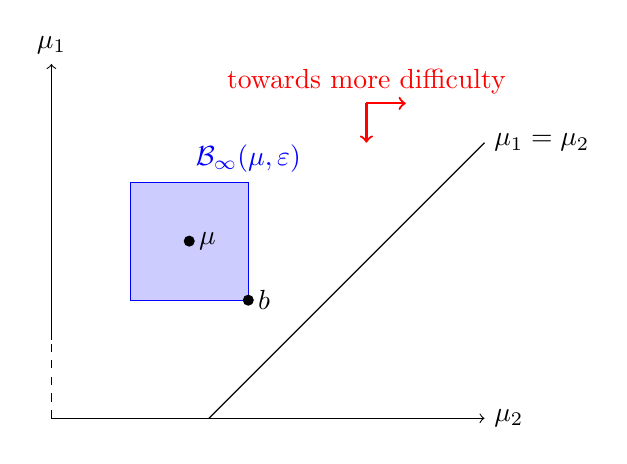
\begin{tikzpicture}
		% Draw axes
		\draw[->] (0,2) -- (5.5,2) node[right] {$\mu_2$}; % x-axis
		\draw[->] (0,3) -- (0,6.5) node[above] {$\mu_1$}; % y-axis
		\draw[dashed] (0,2) -- (0,3);
		% Draw the line y = x
		\draw (2,2) -- (5.5,5.5) node[right] {$\mu_1=\mu_2$};
		% Fill and draw square with vertices (1,1), (2,1), (1,2), (2,2)
		\filldraw[fill=blue!20, draw=blue] (1,3.5) -- (2.5,3.5) -- (2.5,5) -- (1,5) -- cycle;
		\node at (2.5,5) [above] {{\color{blue}$\mathcal{B}_\infty(\bm\mu,\varepsilon)$}};
		\fill (1.75,4.25) circle (2pt) node[right] {$\bm \mu$};
		\fill (2.5,3.5) circle (2pt) node[right] {$\bm b$};
		\draw[->,red,thick] (4,6) -- (4.5,6);
		\draw[->,red,thick] (4,6) -- (4,5.5);
		\node at (4,6) [above] {{\color{red}towards more difficulty}};
	\end{tikzpicture}}
	\caption{$\bm b$ satisfying $\overline{T}^\star(\mathcal{B}_\infty(\bm\mu,\varepsilon))=T^\star(\bm b)$}
	\label{fig:box}
\end{figure}

We display in Figure~\ref{fig:box} a representation of what happens in two-armed BAI.
As long as $\mu_1>\mu_2$, bringing $\mu_1$ down and $\mu_2$ up can only make the problem harder.
If $\varepsilon$ is small enough that all the instances in $\mathcal{B}_\infty(\bm\mu,\varepsilon)$ have the same answer, then the instance on the corner of $\mathcal{B}_\infty(\bm\mu,\varepsilon)$ closest to the line $\mu_1=\mu_2$ is strictly more difficult than all the others.
That means that sampling enough to solve it is enough to solve all the other instances.



